\section{Node Flipping}

The Zhang and Shasha edit distance algorithm is specifically given for ordered trees, that is, the order of child nodes is taken to be significant. In attack trees without sequential conjunction, the order of nodes is not given to be significant~\cite{mauw_foundations_2006,jhawar_attack_2015}. This results in an issue where trees with identical, but unordered nodes are given to have a high edit distance. This is shown in Figure~\ref{fig:nodeflipping}, where two trees with identical information but different node order are given to have a distance of 2. This is due to the fact that the Zhang and Shasha algorithm is not designed to handle unordered trees. Zhang and Jiang have shown that the tree edit distance problem for unordered trees is an MAX SNP-hard~\cite{zhangMAXSNPhardResults1994}. We suggest a novel method for handling tree edit distance in unordered attack trees by taking advantage of the inherent structure of attack trees.


\begin{figure}
    \begin{subfigure}{.45\linewidth}
        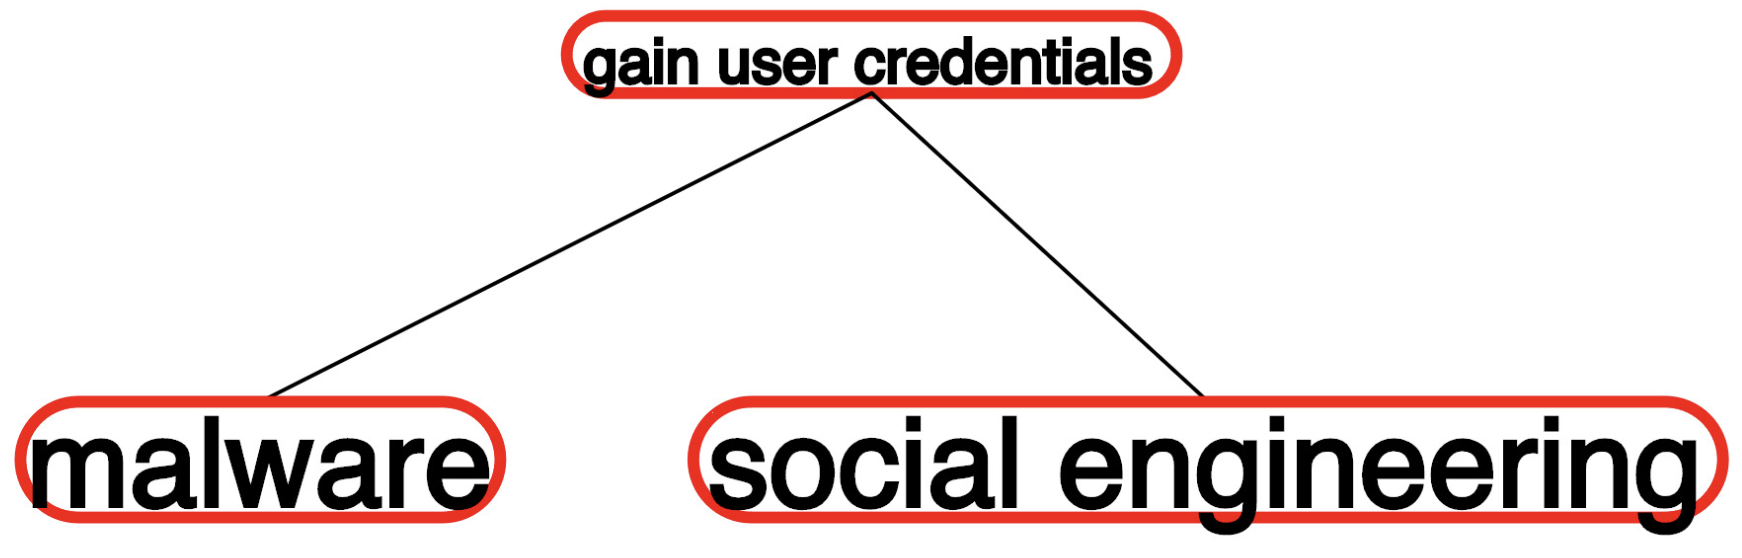
\includegraphics[width=\linewidth]{img/NodeFlip1.png}
    \end{subfigure}
    \begin{subfigure}{.45\linewidth}
        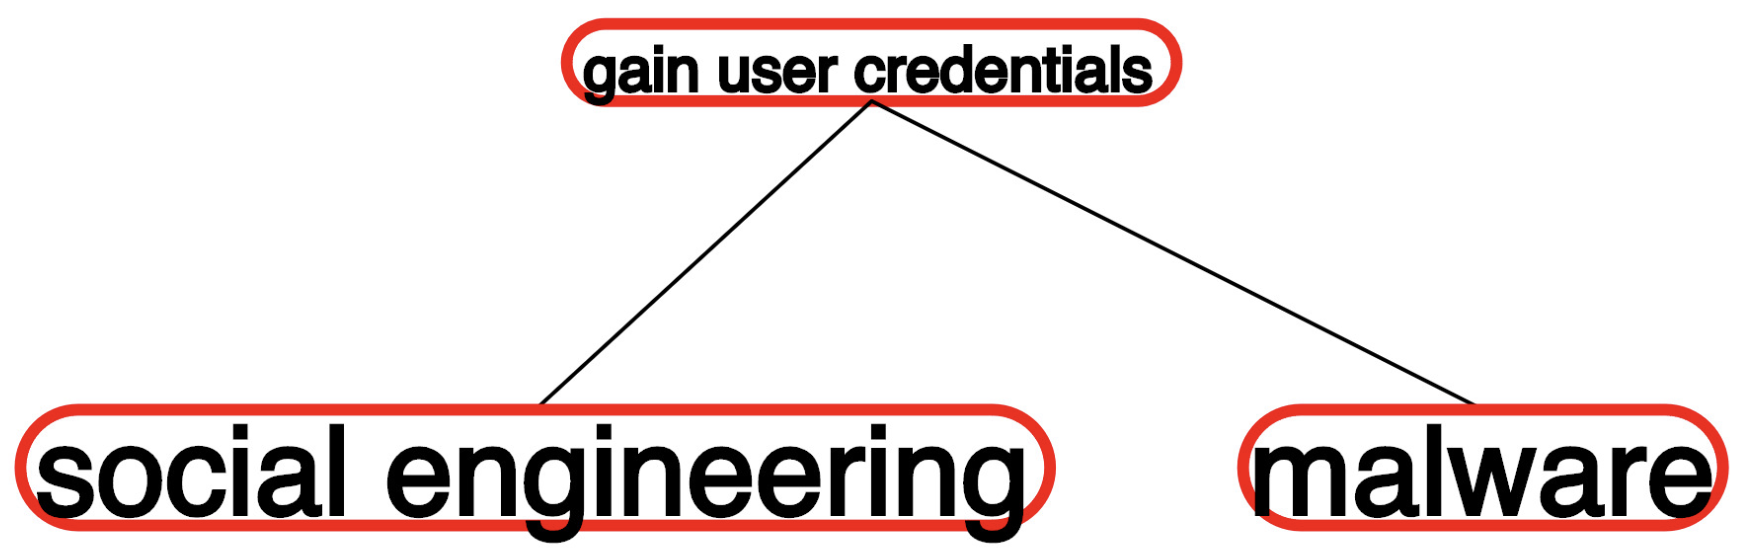
\includegraphics[width=\linewidth]{img/NodeFlip2.png}
    \end{subfigure}
    \caption{Two attack trees (subtrees of the example in Figure~\ref{fig:tartgetAT}) with identical information but different node order. These trees would evaluate to have a distance of 2 (two replacement operations).}
    \label{fig:nodeflipping}
\end{figure}

Attack trees, by virtue of their construction, tend to be organized in levels of abstraction. That is, with each new level of an attack tree, the nodes are given to be more specific than the nodes in the previous level. This is shown in Figure~\ref{fig:tartgetAT}, where the root node is given to be the most abstract (as the overall goal), while the leaf nodes are the most concrete (as the individual actions). From this, we find siblings in an attack tree to be on the same level of abstraction. As such, the order of siblings can be changed without affecting the meaning of the attack tree. By checking the order of sibling sets between the two attack trees




\subsection{Semantic mapping}

Zhang and Shasha motivate and validate their approach by creating a node mapping between the two trees (source and target)~\cite{zhang_simple_1989}. How this mapping is created was not a contribution of that work; however, simple rules for defining mappings based on node placement were included. For example, two nodes could only be mapped if they shared the same placement in terms of parents and siblings. A left-most sibling could not be mapped to a right-most sibling, even if they were the same node. This is part of the reasoning applied to establish that creating this mapping, and thus defining optimal tree-edit distance for unordered trees is an MAX SNP-hard problem~\cite{zhangMAXSNPhardResults1994}.

We adapt the idea of a mapping to instead map nodes based on a comparison of semantic label embeddings. Starting with the root nodes of both source and target trees, we create a matrix of all semantic similarities between the children of these nodes. Starting with the two nodes with the highest label semantic similarity, we map those two nodes together and remove the row and column corresponding to that value from the similarities matrix. Finally, we reorder the children in each tree such that mapped nodes have the same left-wise index. We then repeat this process until the similarities matrix is empty. We then repeat this process for all newly added mappings. This process is shown in Algorithm~\ref{alg:sibling_reorder}. It is a top down algorithm, starting from the root node and working down to the leaf nodes.

This methodology is not guaranteed to return smaller edit distance. If it were, this would represent a polynomial approximate solution to an MAX SNP-hard problem. We can construct a counter example by considering two trees with some identical subtree. If prior to the mapping the parent nodes of these subtrees were in the correct order such that these identical subtrees would be matched by the Zhang and Shasha algorithm, and the process of creating the semantic mapping caused the parent nodes of these identical subtrees to be placed out of order, the tree edit distance would increase as a result of our mapping step, as the previous matching operations (which are given to not have a cost) would no longer occur in the Zhang and Shasha algorithm, and would likely be replaced with a large series of add and remove operations (which each incur a cost). However, this scenario is only possible if the root nodes of these identical subtrees are not semantically mapped together, which is highly unlikely to occur in practice. This potential could be mitigated by calculating the tree edit distance twice: once with semantic node remapping and once without, to check that the node mapping has not increased edit distance. Such a step would not increase the computational complexity of the overall calculation, but would ensure that the worse case scenario does not occur.





\begin{algorithm}
    \caption{An algorithm to reorder siblings based on semantic similarity}
    \label{alg:sibling_reorder}
    \begin{algorithmic}
        \State Two attack trees $T_1$ and $T_2$ according to Definition~\ref{def:attack-tree} with $a$ and $b$ total nodes respectively
        \State $M$ is the mapping of nodes between $T_1$ and $T_2$ \Comment{We give $m[0]$ and $m[1]$ to be the source and target nodes of a mapping for $m \in M$}
        \State $M \gets T_1[a]\mapsto T_2[b]$\Comment{Root nodes are always mapped}
        \For{$m \in M$}

        \State $D \gets []$ \Comment{Matrix of semantic similarity values}
        \For{left-wise index $i$ in $m[0].\text{children}$}
            \For{leftwise index $j$ in $m[1].\text{children}$}
                \State $D[i][j] \gets$ 
                \State$\text{  }\text{  }\text{  }\text{  }\text{  }\text{  }\text{  }\text{  }\text{  }\delta(m[0].\text{children}[i].\text{label}, m[1].\text{children}[j].\text{label})$
            \EndFor
        \EndFor
        \State $M_t \gets \emptyset$ \Comment{Temporary set of mappings} 
        \While{$D$ is not empty}
            \State $i, j \gets \text{argmax}(D)$ \Comment{Largest value in $D$}
            \State $M_t \gets M_t \cup m[0].\text{children}[i]\mapsto m[1].\text{children}[j]$
            \State $D \gets D - i$ \Comment{Remove row $i$}
            \State $D \gets D - j$ \Comment{Remove column $j$}
        \EndWhile
        \For{$p$ in $M_t$}
            \If{indicies $i$, $j$ of $p$ are not equal}
                \State{Swap nodes $i$ and $j$ \textbf{in $T_1$}}
            \EndIf
        \EndFor
        \State $M \gets M \cup M_t$
        \EndFor
    \end{algorithmic}
    \end{algorithm}


    \subsection{Ordered Subtrees}

    As we have discussed in Sections~\ref{sec:background}~and~\ref{sec:refinement-awareness}, there are components of attack trees which can be given to be ordered; namely, \SAND\ attack trees~\cite{jhawar_attack_2015}. While these attack trees are out of scope for our definition and contribution, they are a common extension on the attack tree formalism~\cite{lallieReviewAttackGraph2020}. If a \SAND\ node exists within an attack tree, Algorithm~\ref{alg:sibling_reorder} can be modified to check the relationship between children of nodes and to directly map ordered nodes together regardless of label semantic similarity. As stated previously, this is out of scope for our contribution; the validation and testing of such an approach will have to be attended to in a future work.